\documentclass[12pt, a4paper, oneside]{article} 

\usepackage{czech} % nastavení češtiny
\usepackage[center]{caption} 
\usepackage[utf8]{inputenc}
\usepackage{wrapfig} % nastavení obtékání textu
\usepackage{graphicx,amsmath} % nastavení grafiky, matematiky
\usepackage{subfig} % více obrázků vedle sebe 
\usepackage{float}
\usepackage{amsmath}
\usepackage{amssymb}
\usepackage{bbding}
\usepackage{enumitem}
\usepackage{breakurl}
\usepackage{pdflscape}
%\usepackage{indentfirst}

\usepackage{tocloft} %přidá tečky do obsahu ke kapitolám /sekcím 
\renewcommand{\cftsecdotsep}{\cftdotsep}

\usepackage[bookmarksopen,colorlinks,plainpages=false,linkcolor=black,urlcolor=blue,citecolor=black,filecolor=black,menucolor=black,unicode=true]{hyperref}

\urlstyle{rm}
%bookmarksopen -- open up bookmark tree 
%colorlinks -- zbarví odkazy (implicitně orámovaný nezbarvený text)
%urlcolor -- barva odkazů (implicitně magenta) 
%linkcolor=black -- barva odkazů v obsahu (implicitně red)


\usepackage{listings}
\usepackage{color}
%\usepackage{minted}
\definecolor{lightgray}{RGB}{240,240,240}
\definecolor{darkgray}{rgb}{.4,.4,.4}
\definecolor{purple}{rgb}{0.65, 0.12, 0.82}
\definecolor{darkgreen}{RGB}{0,150,0}

%\usemintedstyle{perldoc}
%\newminted{js}{linenos=true, bgcolor=lightgray}

\lstdefinelanguage{JavaScript}{
  keywords={typeof, new, true, false, catch, function, return, null, catch, switch, var, if, in, while, do, else, case, break, for},
  keywordstyle=\color{blue}\bfseries,
  ndkeywords={class, export, boolean, throw, implements, import, this},
  ndkeywordstyle=\color{blue}\bfseries,
  identifierstyle=\color{black},
  sensitive=zr,
  comment=[l]{//},
  morecomment=[s]{/*}{*/},
  commentstyle=\color{darkgreen}\ttfamily,
  stringstyle=\color{red}\ttfamily,
  morestring=[b]',
  morestring=[b]"
}

\lstset{
   backgroundcolor=\color{lightgray},
   extendedchars=true,
   basicstyle=\footnotesize\ttfamily,
   showstringspaces=false,
   showspaces=false,
   numbers=left,
   numberstyle=\footnotesize,
   numbersep=9pt,
   tabsize=2,
   breaklines=true,
   showtabs=false,
   aboveskip=5mm,
   belowskip=7mm,
   captionpos=b
}

\renewcommand{\listingscaption}{Příklad}
\renewcommand{\listoflistingscaption}{Příklady}

% \usepackage{parskip} -- zapne americké odstavce v celé práci

\addtolength{\textwidth}{-2mm} 
\addtolength{\hoffset}{4mm}  % posun textu kvůli kroužkové vazbě  

\setlength{\intextsep}{5mm} % nastavení mezery okolo obrázků

% nastavení příkazu >\figcaption pro popis čehokoli, jako by to byly obrázky 
\makeatletter   
\newcommand\figcaption{\def\@captype{figure}\caption}
\makeatother

\renewcommand\refname{Literatura} 
%\def\bibname{PŘÍLOHA D: Reference}
%\renewcommand\bibname{PŘÍLOHA D: Reference}
% přejmenuje anglický název Reference na české Literatura


%\makeindex % příprava pro výrobu indexu (jestli ho chcete)

%%    VLNKA <fileinput>  KkSsVvZzOoUuAaIi        
% Defaultni  koncovka pro <fileinput> je  ".tex"
%FIXME: haze error
%\cstieon % Vypne chovani vlnky jako tvrde mezery v matematickem rezimu

%%%%%%%%%%%%%%%%%%%%%%%%%%%%%%%%%%%%%%%%%%%%%%%%%%%%%%%%%%%%%%%
%V PROSTŘEDÍ ROVNIC SE NESMÍ VYSKYTOVAT PRÁZDNÝ ŘÁDEK
%
%PROGRAMY VLNKA A CSINDEX SE MUSÍ SPUSTIT SAMOSTATNĚ
%%%%%%%%%%%%%%%%%%%%%%%%%%%%%%%%%%%%%%%%%%%%%%%%%%%%%%%%%%%%%%%

% definice příkazů 
\newcommand{\D}{\medskip \noindent} % nový odstavec v "americkém" formátování 
\newcommand{\B}{\textbf} %tučné písmo
\newcommand{\A}{\mathbf} %tučné písmo v matematickém režimu
\newcommand{\TO}{\ensuremath{\boldsymbol\Omega}} % tučný znak velké omega -- pro ohmy
\newcommand{\I}{\index}  % vytváří položku indexu (asi nepoužijete)
\newcommand{\Deg}[1][]{\ensuremath{{#1}^\circ}} % vysází značku stupně Celsia
\newcommand{\Def}{\footnotesize Definice: \normalsize}
\newcommand{\Pos}{\footnotesize Experiment: \normalsize}
\newcommand{\Odv}{\footnotesize Odvození: \normalsize}
\newcommand{\Vym}{\footnotesize Vymezení pojmu: \normalsize}
\newcommand{\Ob}{obrázek }
\newcommand{\It}{\textit}  % kurzíva
\newcommand{\M}{\mathrm}   % v prostředí rovnic nastaví normální písmo (místo kurzívy ) 
\newcommand{\F}{\footnotesize} % zmenšená velikost písma
\newcommand{\N}{\normalsize} % normální velikost písma
%\newcommand{\U}{\underline}  % podtržené písmo
\newcommand{\e}{\ensuremath} 
\newcommand{\Has}{\textcolor{green}{\CheckmarkBold}}
\newcommand{\NoHas}{\textcolor{red}{\XSolidBrush}}
% další příkaz se aplikuje, pouze, když jste v matematickém režimu

%\hyphenation{Pusť-me pla-tí hod-no-ty do-sa-dí-me za-da-né dal-ším}
% dělení slov, kdyby implicitní nevyhovovalo

\linespread{1.3} 
% řádkování 1,5x  
% použijete podle situace  

\unitlength=1mm % nastavení volby jednotek 

% konec hlavičky
%%%%%%%%%%%%%%%%%%%%%%%%%%%%%%%%%%%%%%%%%%%%%%%%%%%%%%%%%%%%%%%%%%%
%%%%%%%%%%%%%%%%%%%%%%%%%%%%%%%%%%%%%%%%%%%%%%%%%%%%%%%%%%%%%%%%%%%

\begin{document} % začátek textové části 

% titulní strana
\pagestyle{empty} % vynechá číslování
 
\voffset = -20mm % posun začátku textu výš
\enlargethispage{60mm} % zvětší oblast tisku pro tuto stránku   

\begin{center}
 
\Large \B{STŘEDOŠKOLSKÁ ODBORNÁ ČINNOST}

\vspace{60mm}

\Huge %\LARGE
\B{MultiROM} \\
\LARGE
\B{Nástroj pro instalaci více operačních systému na mobilní zařízení}
% na titulní straně může být stručnější, pokud je to potřeba  

\Large

\vspace{90mm}


\B{Vojtěch Boček} \\

\vspace{40mm}

\B{Brno 2014}


\end{center}

\newpage % konec titulní strany 
%%%%%%%%%%%%%%%%%%%%%%%%%%%%%%%%%%%%%%%%%%%%%%%%%%%%%%%%%%%%%%%%%%%%%%%%%%%

% vnitřní titulní strana
\voffset = -20mm % posun začátku textu výš
\enlargethispage{60mm} % zvětší oblast tisku pro tuto stránku   

\begin{center}

\Large \B{STŘEDOŠKOLSKÁ ODBORNÁ ČINNOST}  \\
\vspace{10mm}
 \normalsize 
\B{Obor SOČ: 18. Informatika}% číslo a název -- vyplníme spolu 

\vspace{45mm}

\Huge
\B{MultiROM} \\
\LARGE
\B{Nástroj pro instalaci více operačních systému na mobilní zařízení}
\end{center}
\large

\vspace{50mm}


\begin{tabbing}
\hspace{10mm} \= \hspace{30mm}  \=   \kill % nastavení zarážek 
  \> \B{Autor:}  \> \B{Vojtěch Boček}        \\[8mm] 
  \> \B{Škola:}   \> \B{SPŠ a~VOŠ technická, }     \\
  \>              \> \B{Sokolská 1, 602 00 Brno}    \\[8mm]
\end{tabbing}

\vspace{20mm}

\begin{center}
\B{Brno 2014}

\end{center}
\normalsize
%%%%%%%%%%%%%%%%%%%%%%%%%%%%%%%%%%%%%%%%%%%%%%%%%%%%%%%%%%%%%%%%%%%%%%%%%%%
\newpage  % Prohlášení o autorství  
\voffset = 0mm % posun začátku textu zpět

~ % musí to tu být, aby fungovala svislá mezera

\vspace{10mm}

\section*{Prohlášení}

Prohlašuji, že jsem svou práci vypracoval samostatně, použil jsem pouze podklady (literaturu, SW atd.) citované v~práci a~uvedené v~přiloženém seznamu a~postup při zpracování práce je v~souladu se zákonem č. 121/2000 Sb., o~právu autorském, o~právech souvisejících s~právem autorským a~o~změně některých zákonů (autorský zákon) v~platném znění. 
 
\vspace{20mm} 
 
\noindent V~Brně  dne: 6.3.2014 \hspace{50mm}                 podpis:   
 

%%%%%%%%%%%%%%%%%%%%%%%%%%%%%%%%%%%%%%%%%%%%%%%%%%%%%%%%%%%%%%%%%%%%%%%%%%%
\newpage   % Poděkování -- nepovinné 

~ % musí to tu být, aby fungovala svislá mezera
\vspace{100mm}

\section*{Poděkování}
Děkuji Jakubu Streitovi za rady, obětavou pomoc, velkou trpělivost a~podnětné připomínky poskytované během práce na tomto projektu, Martinu Vejnárovi za informace o~programátoru Shupito, panu profesorovi Mgr. Miroslavu Burdovi za velkou pomoc s~prací a~v~neposlední řadě Bc. Martinu Foučkovi za rady a~pomoc při práci s~Qt Frameworkem. Dále děkuji organizaci DDM Junior za poskytnutí podpory.
 

%%%%%%%%%%%%%%%%%%%%%%%%%%%%%%%%%%%%%%%%%%%%%%%%%%%%%%%%%%%%%%%%%%%%%%%%%%%
\newpage   % Anotace 
~ % musí to tu být, aby fungovala svislá mezera
\vspace{-20mm}

\section*{Anotace}

%MultiROM is one-of-a-kind multi-boot mod for Nexus 7. It can boot any Android ROM as well as other systems like Ubuntu Touch, Plasma Active, Bohdi Linux or WebOS port.Besides booting from device's internal memory, MultiROM can boot from USB drive connected to the device via OTG cable. The main part of MultiROM is a boot manager, which appears every time your device starts and lets you choose ROM to boot. You can see how it looks on the left image below and in gallery. ROMs are installed and managed via modified TWRP recovery. You can use standard ZIP files to install secondary Android ROMs, daily prebuilt image files to install Ubuntu Touch and MultiROM even has its own installer system, which can be used to ship other Linux-based systems.

Tato práce popisuje modifikaci pro mobilní zařízení s operačním systémem Google Android, která umožňuje instalaci více operačních systémů vedle sebe, podobně jako na PC. Může to být pouze několik různých verzí OS Google Android, ale i úplně jiné systémy - například právě se vyvíjejicí Ubuntu Touch a další.

Možnost provozovat více operačních systému na jedno zařízení je užitečná spíše pro pokročilé uživatel, podobně jako na stolních počítačích, nicméně počet aktivních uživatelů dokazuje, že zájem o tuto modifikaci rozhodně existuje.


%Tato práce popisuje komplexní sadu nástrojů pro vývoj a~ovládání libovolného zařízení schopného komunikovat po sériové lince nebo TCP socketu.

%Protože se nejedná o~jednoduchou aplikaci ani o~jednostranně zaměřenou sadu nástrojů, protože se navíc celá sada průběžně rozrůstá a~protože je rozsah a~záběr použití všech funkcí a~modulů této sady příliš velký, nelze ji stručně popsat v~omezeném prostoru anotace.

%Pro získání ucelenější představy o~tom, co vše lze pomocí sady Lorris dosáhnout, prosím nahlédněte do \hyperref[uvod]{úvodu práce}.

%Aplikace zastřešuje několik modulů. Každý modul je určen pro specifickou činnost -- parsování a zobrazování dat, programování mikročipů atd.

%Hlavním přínosem tohoto softwarového balíku je, že urychluje, zpřehledňuje a~hlavně výrazně zjednodušuje vývoj a~testování aplikací pro mikročipy, typicky programování a~řízení různých druhů robotů.

%\D \B{Klíčová slova:} analýza binárních dat, programování a~řízení robotů, vývoj pro mikrokontroléry, programování mikročipů

\addtolength{\textheight}{30mm} % prodlouží následující stránku

%%%%%%%%%%%%%%%%%%%%%%%%%%%%%%%%%%%%%%%%%%%%%%%%%%%%%%%%%%%%%%%%%%%%%%%%%%%
\newpage
\pagestyle{plain}

\setlength{\voffset}{-20mm} % posune text/obrázek na této stránce nahoru
\setcounter{page}{1}  % nastaví čítač stránek znovu od jedné

\tableofcontents  % vysází obsah

\addtolength{\textheight}{-30mm} % zkrátí následující stránku
%%%%%%%%%%%%%%%%%%%%%%%%%%%%%%%%%%%%%%%%%%%%%%%%%%%%%%%%%%%%%%%%%%%%%%%%%%%
\newpage
\setlength{\voffset}{0mm} % posune text/obrázek na této stránce, kam patří
%\pagestyle{headings} % znovu zapne číslování
\pagestyle{plain}

%
% Motivace 
\section*{Úvod}
\addcontentsline{toc}{section}{Úvod} % přidá položku úvod do obsahu
\label{uvod}



\section{Motivace}
Abych mohl vysvětlit důvod, proč je multi-boot na mobilních zařízeních užitečný, musím nejdříve upozornit na možnosti, které tato zařízení mají.

Tablety a telefony s platformou Google Android lze narozdíl od jiných systémů relativně snadno upravovat. Uživatelé na nich mohou získat přístup k tzv. superuživateli\footnote{Uživatel, který má práva přistupovat a měnit všechny části systému, je možné ho připodobnit k uživateli \It{Administrátor} v MS Windows. V Linuxu se jmenuje \It{root}.} a dále pak upravovat software na zařízení jakýmkoliv způsobem chtějí. Toto společně s faktem, že velká část OS Android má otevřené zdrojové kódy, vedlo ke vzniku obrovské komunity programátorů a nadšenců, kteří tyto zařízení různými způsoby upravují a vylepšují. Jedním z \uv{produktů} této komunity jsou celé upravené distribuce Androidu, tzv. ROM.

\subsection{Android ROM}
ROM lze přirovnat k distribucím Linuxu, jak je známe ze stolních počítačů. Jejich základem jsou obvykle zdrojové kódy z AOSP\cite{aosp}\footnote{\It{Android Open Source Project} - označení pro otevřenou část zrojových kódů OS Android}, které si autoři upravují podle svých představ - přidávají optimalizace pro zrychlení celého systému, přidávají další možnosti personalizace pro uživatele, mění prvky uživatelského rozhraní a mnoho dalšího. Na zařízeních, která již nejsou podporované výrobcem, mohou být ROM jediným způsobem, jak na ně přinést novější verze OS Android.

ROM často vydávají a spravují pouze jednotlivci, ale existují i projekty s velkým počtem vývojářů i uživatelů, například CyanogenMod\cite{CM}. Ten nedávno překonal hranici 10 milionů uživatelů, oficiálně podporuje přes 200 zařízení a je aktuálně největší upravenou ROM.

\subsection{Další operační systémy}
Kromě Androidu existují i další mobilní operační systémy, například Ubuntu Touch\cite{utouch}, Mozilla Firefox OS\cite{firefoxos} a další. Tyto systémy často použivají zařízení původně prodávaná s Androidem jako testovací, zejména kvůli jejich snadné dostupnosti a relativně nízké ceně. Pro tablet Google Nexus 7 dokonce existuje plná verze Linuxové distribuce Ubuntu, díky které je možné tento tablet po připojení klávesnice a myši používat jako netbook, s většinou programů které známe z PC.

\begin{figure}[H]
\begin{center}
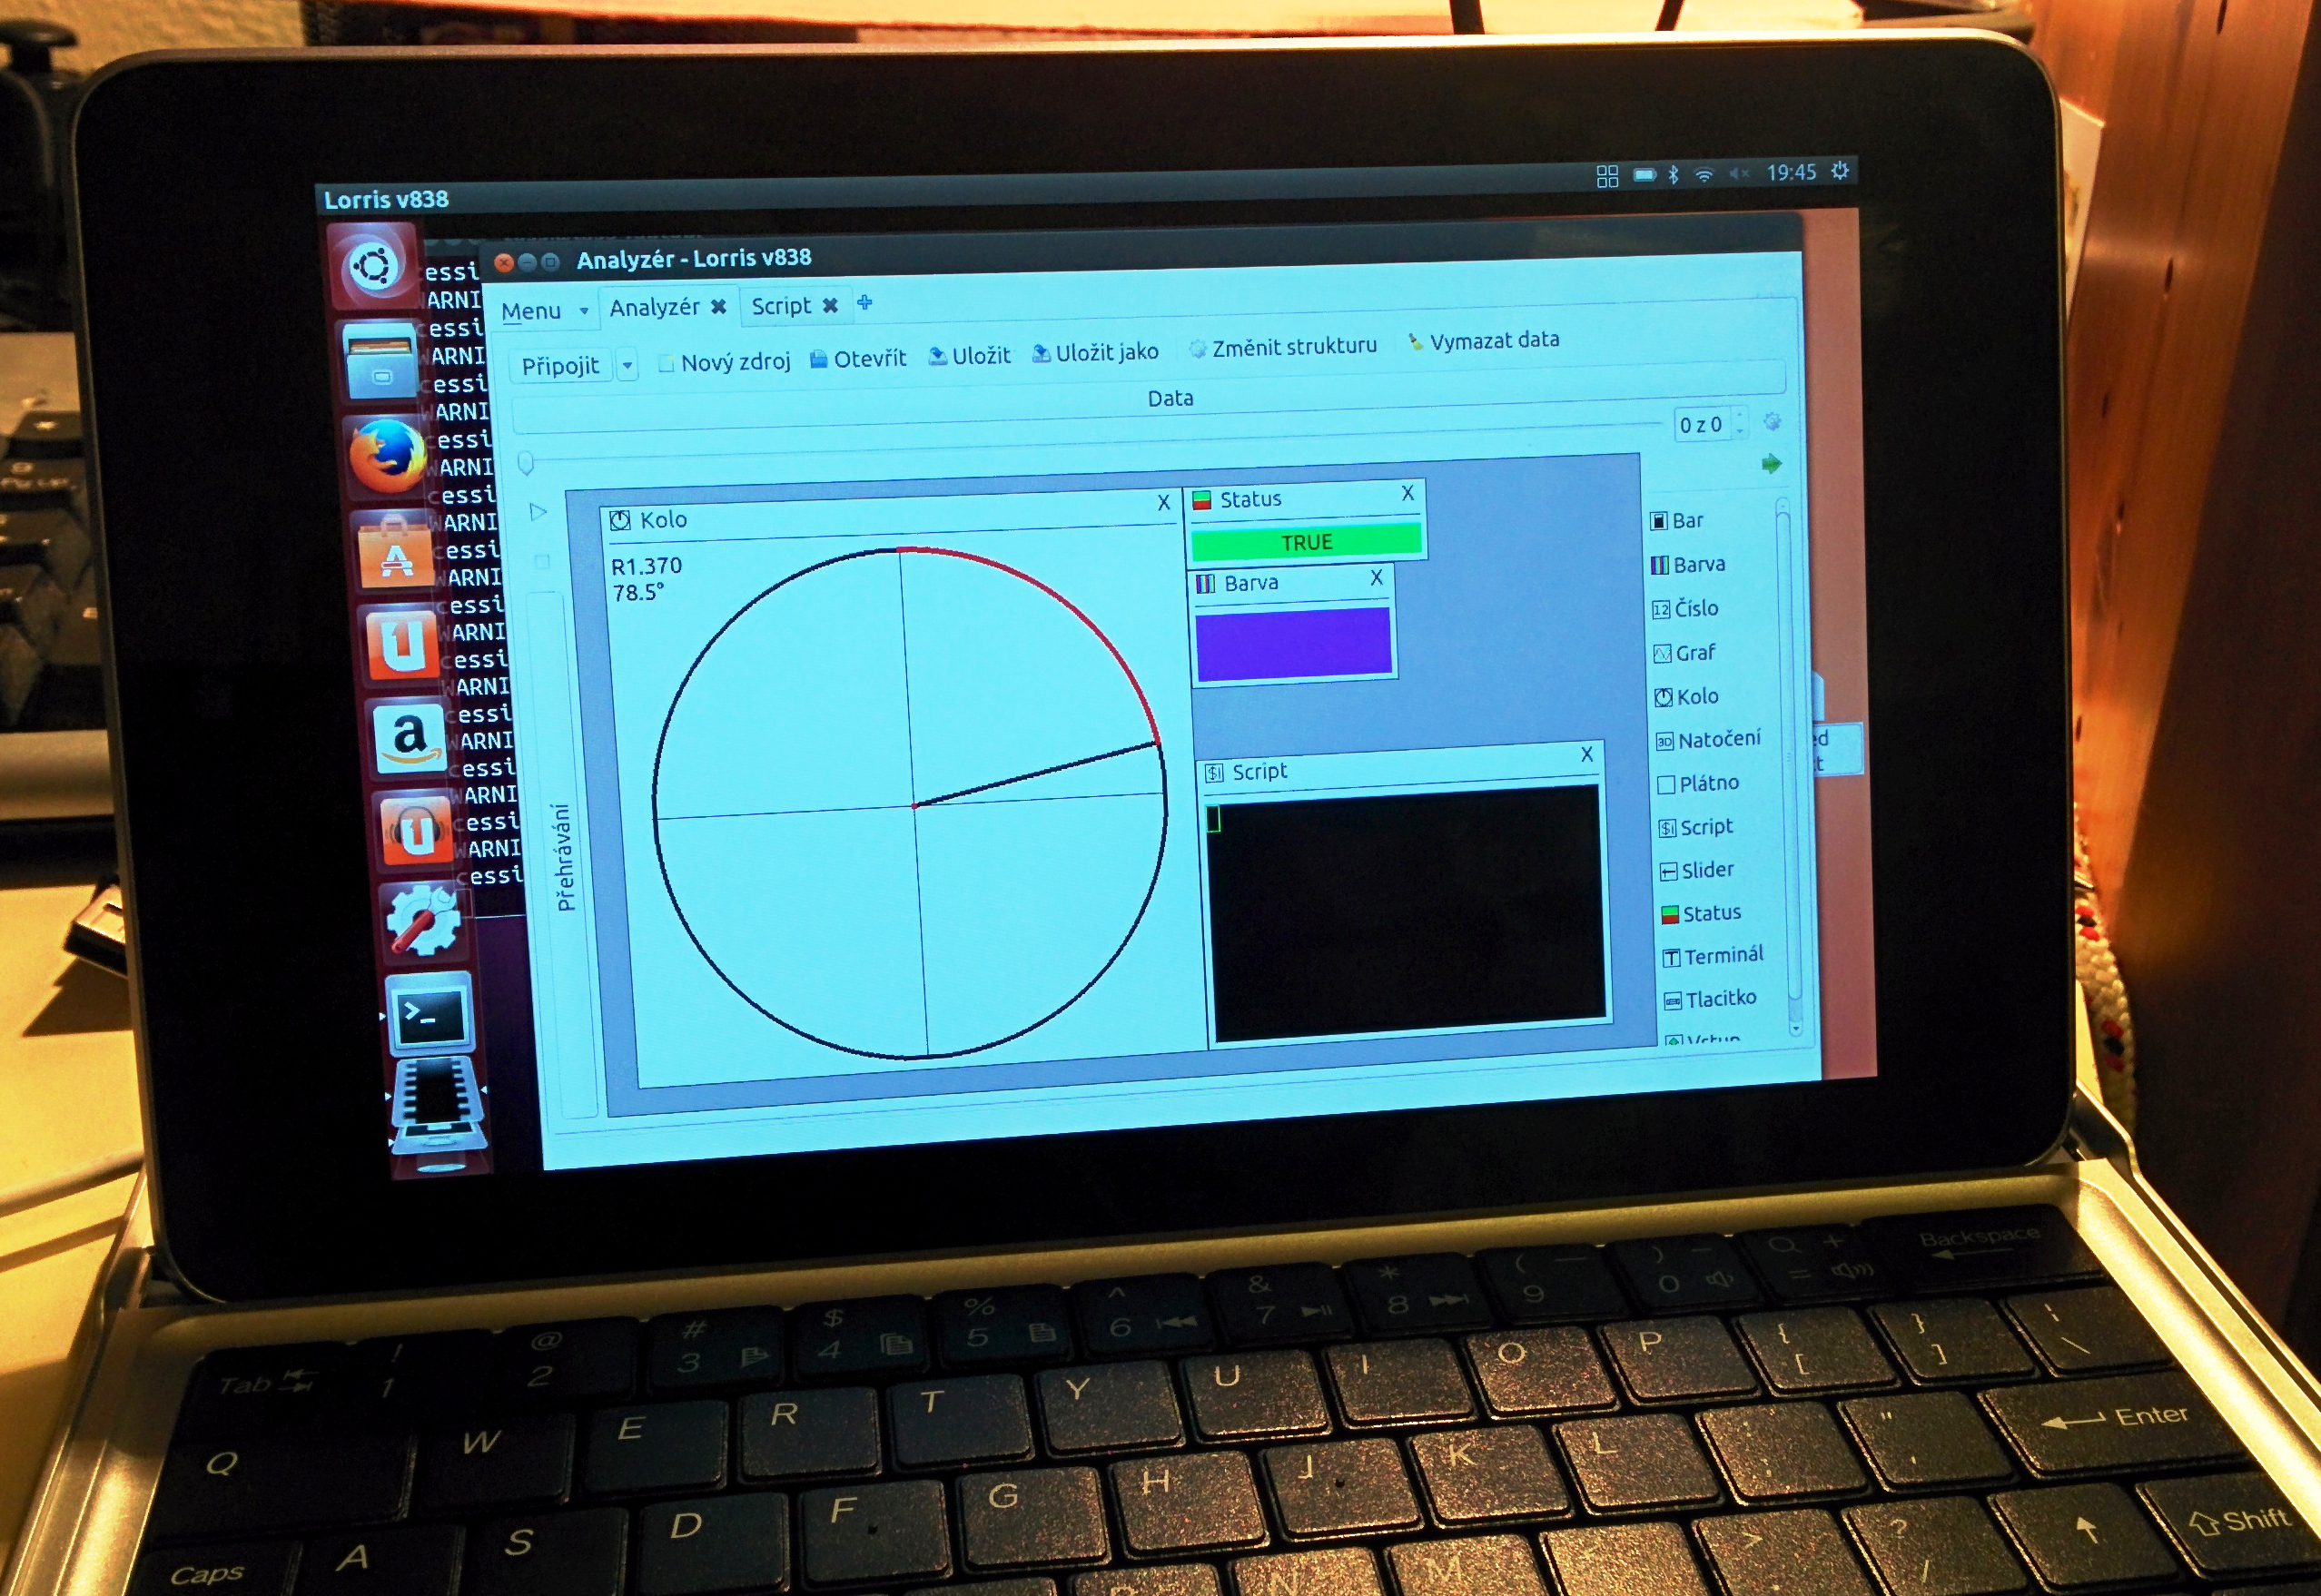
\includegraphics[width=\textwidth]{img/n7_ubuntu.jpg}
\caption{Ubuntu na tabletu Nexus 7 s připojenou klávesnicí}
\label{split_img}
\end{center}
\end{figure}


\subsection{Více systémů na jednom zařízení}
Tyto telefony a tablety tedy ve většině případů (více o této problematice v příloze \uv{\nameref{sec:locked}}) nejsou uzamknuté na jediném, výrobcem vybraném systému a jeho verzi a dokáží podobně jako stolní počítače provozovat více typů a verzí operačních systémů. Chybí jim však možnost mít více systémů nainstalovaných zárověň.



\newpage
\section*{Závěr}
\addcontentsline{toc}{section}{Závěr}



%%%%%%%%%%%%%%%%%%%%%%%%%%%%%%%%%%%%%%%%%%%%%%%%%%%%%%%%%%%%%%%%%%%%%%%%%%%
\newpage
\section*{PŘÍLOHA A:}
\section*{Uzamykání zařízení pouze na určitý systém}
\label{sec:locked}
I když zdrojové kódy OS Android jsou z velké části otevřené, mezi výrobci panuje trend uzamykaní zařízení tak, aby mohli uživatelé používat pouze systém vydaný výrobcem, ať už v zájmu bezpečnosti, zachování určitých vlastností systému (např. předinstalované aplikace často obtěžující uživatele) nebo z prostého nepochopení trhu. V současnosti existuje několik typů uzamknutí zařízení:

\begin{enumerate}
    \item \B{Volně odemykatelné} - uživatel si je může sám odemknout, bez žádných nevýhod oproti uzamknutým zařízením. Tento typ je nejvíce ojedinělý, příkladem jsou zařízení z řady \It{Nexus} vydávané pod záštitou firmy Google.
    
    \item \B{Odemykatelné za registraci} - výrobce provozuje web, který po zadání sériového čísla zařízení vydá odemykací kód. Takto si vytvoří databázi odemknutých zařízení, kterou poté může využít k zamítnutí reklamací (podobné chování nemusí být v souladu s legislativou).
    
    Někteří výrobci při tomto odemknutí smažou klíče pro placený obsah (tzv. DRM\footnote{\It{Digital Rights Management} - systémy navrhnuté pro zabránění nelegálního kopírování digitálního obsahu - hudby, filmů, her apod.}), protože je na odemknutých systémech podle jejich názoru větší nebezpečí nelegálního kopírování obsahu chráněného pomocí DRM.
    
    \item \B{\uv{Edice pro vývojáře}} - výrobce kromě standardní varianty zařízení vydávají verzi, kterou je možné odemknout, buďto za registraci nebo volně. Tyto edice jsou často bezdůvodně dražší anebo nejsou dostupné ve všech zemích, ve kterých je možné koupit standardní variantu. Označení \uv{Developer edition}, které výrobci používají, je v tomto případě mírně zavádějící - zařízení je možné pouze odemknout a kromě této skutečnosti není o nic více přispůsobené vývojářům (části s uzavřeným zdrojovým kódem jsou stále nedostupné a hardware telefonu je rovněž stejný).

    \item \B{Bez možnosti odemknutí} - výrobce neposkytuje žádný způsob jak zařízení odemknout. V naprosté většině případů ale komunita překoná toto omezení a existuje více nebo méně pohodlná možnost neoficiálního odemknutí. Někteří výrobci tomuto odporují a dokonce přidávají vlastnosti kontrolující integritu systému a sledující, zda nebylo uzamknutí prolomeno. Tyto ochrany bývají často také překonány.
    
\end{enumerate}

\newpage
 \section*{PŘÍLOHA E:}
 \begin{thebibliography}{99}
\addcontentsline{toc}{section}{PŘÍLOHA E: Reference}
 %% 99 znamená, že maximální délka čísla literatury jsou dva znaky
% seznam samozřejmě změníte podle svého, tohle je pouze ukázka formátování

    \bibitem{aosp} \It{Android Open Source Project} \\
    \url{http://source.android.com/}\\
    (Stav ke dni 19.\,1.\,2014)

    \bibitem{CM} \It{CyanogenMod} \\
    \url{http://www.cyanogenmod.org/}\\
    (Stav ke dni 19.\,1.\,2014)

    \bibitem{utouch} \It{Ubuntu Touch} - Ubuntu on phones \\
    \url{http://www.ubuntu.com/phone}\\
    (Stav ke dni 21.\,1.\,2014)

    \bibitem{firefoxos} \It{Firefox OS}\\
    \url{http://www.mozilla.org/cs/firefox/os/}\\
    (Stav ke dni 21.\,1.\,2014)


\end{thebibliography}

\newpage
\section*{PŘÍLOHA G:}
~
\addcontentsline{toc}{section}{PŘÍLOHA G: Seznam obrázků}
\listoffigures   % seznam obrázkù 

\end{document}
